\chapter{Programmets brugergrænseflade}
I dette kapitel vil programmet grafiske brugergrænseflade blive beskrevet.

\section{Login brugergrænseflade}
\begin{wrapfigure}{r}{0.5\textwidth}
    \label{img:login_interface}
    \vspace{-20pt}
    \begin{center}
        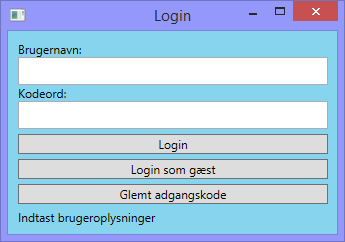
\includegraphics[width=0.48\textwidth]{UI/Login_Window_Empty_Fields.png}
    \end{center}
    \vspace{-15pt}
    \caption{Login interface}
\end{wrapfigure}

Login brugergrænsefladen (Figur \ref{img:login_interface}) er opstartsvinduet, og giver brugerne mulighed for at logge ind.
Formålet med dette er, at programmet skal kende identiteten af den person som anvender programmet.
Login knappen (samt at trykke på ``Enter''/``Return''-knappen mens tekstfelterne er i fokus), udfører et login. 
Forudsagt at brugeroplysninger angivet er korrekte, eller vises en passende fejlbesked.
Man kan også logge ind som en gæste bruge, som har reducerede tilladelser. 
Den kan bruges, hvis man vil tjekke noget infomation hurtigt, og ikke vil til at logge ind, da det tager tid.
Dette udføres ved at trykke på ``Login som gæst''-knappen. 

Efter fuldført login åbens et passene hovedvindue, med funktionaliteter i henhold til tabel \ref{tab:permissions}.

% LaTeX tabel som viser alle brugerniveauer og deres muligheder efter login.
% http://bit.ly/1kToHZ3 to edit raw table
\begin{table}
    \colorlet{shadecolor}{gray!40}
    \rowcolors{1}{white}{shadecolor}
    \begin{tabular}{l|llllll}
    ~                        & Gæst & Støttemedlem & Medlem & Elev & Underviser & Administrator \\ \hline
    Personlig forside        & ~    & ~             & \ding{51}     & \ding{51}    & \ding{51}          & \ding{51}             \\
    Se begivenheder          & \ding{51}    & \ding{51}             & \ding{51}      & \ding{51}    & \ding{51}          & \ding{51}             \\
    Tilmeld begivenheder     & ~    & ~	             & \ding{51}      & \ding{51}    & \ding{51}          & \ding{51}             \\
    Opret begivenheder       & ~    & ~             & ~      & ~    & \ding{51}          & \ding{51}             \\
    Se sejlture              & \ding{51}    & \ding{51}             & \ding{51}      & \ding{51}    & \ding{51}          & \ding{51}             \\
    Opret sejltur            & ~    & ~             & \ding{51}      & \ding{51}    & \ding{51}          & \ding{51}             \\
    Se logbøger              & \ding{51}    & \ding{51}             & \ding{51}      & \ding{51}    & \ding{51}          & \ding{51}             \\
    Opret logbog             & ~    & ~             & \ding{51}      & \ding{51}    & \ding{51}          & \ding{51}             \\
    Svar på logbog           & ~    & ~             & ~      & ~    & ~          & \ding{51}             \\
    Se undervisningstimer    & ~    & ~             & ~      & \ding{51}    & \ding{51}          & \ding{51}             \\
    Opret undervisningstimer & ~    & ~             & ~      & ~    & \ding{51}          & \ding{51}             \\
    \end{tabular}
    \caption{Tabel over alle brugerniveauer og deres tilladte funktioner.}\label{tab:permissions}\fixme{Måske skal denne tabel lige laves lidt om, enten indholdet, eller hvordan det virker i programmet.}
\end{table}

\section{Primære brugergrænseflade}
Det primære vindue tilgåes via login vinduet, som er det der starter ved programstart, eller logud. 
Der findes 4 vinduer, forskellen mellem dem er hvilke tabs der er aktive. 
I hver tab findes der en funktionalitet, samlet set findes følgende tabs:
\begin{itemize}% Denne skulle måske relatere til tabel tab:permission
    \item Forside
    \item Undervisning
    \item Begivenheder
    \item Medlemmer
    \item Både
\end{itemize}

Via hver af disse tabs, vil der være adgang til programmet forskellige funktionaliteter.
Der er også en log ud knap, som bruges til at vende tilbage til loginvinduet, således en anden bruger kan anvende systemet.
Programmet er lavet til at køre i opløsningen 1024x720 pixels.
Denne opløsning er valgt for at understøtte alt fra bærbare, med opløsninger som 1366x768 pixels i et vindue, og op til FullHD (1920x1080 pixels) osv.
Programmet har et lyst farveskema, men farverne hvid og en lys blå som hovedfarver (\#87D4EE).

\section{UserControls}
Der anvendes UserControls til at kode både brugergrænsefladen og den tilhørende code behind.


\subsection{DateTimePicker}\label{subsec:DateTimePicker}

\begin{wrapfigure}{r}{0.5\textwidth}
    \label{img:DateTimePicker}
    \vspace{-20pt}
    \begin{center}
        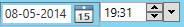
\includegraphics[width=0.48\textwidth]{Screenshots/DateTimePicker.png}
    \end{center}
    \vspace{-15pt}
    \caption{DateTimePicker}
    \vspace{-30pt}
\end{wrapfigure}

\textbf{Formål}: Denne Usercontrol, er lille i forhold til de andre der findes i programmet.
Den bruges når der skal vælges et tidspunkt som både indeholder en dato og et tidspunkt. 
Der findes en DateTimePicker i extended WPF toolkit, men da der blev opdaget en underlig fejl ved denne, blev det besluttet at en usercontrol, som gruppen selv kunne programmere, ville være bedre. 

\textbf{BrugerGrænseflade}: Den består af en DatePicker, og en TimePicker som findes i extended WPF toolkit.

\textbf{Code-Behind}: De to værdier man skriver i henholdsvis DatePickeren og TimePickeren, skal samles i en enkelt værdi som kan tilgås vha. usercontrollen. 
Dette er gjort ved at lave et property der kaldes for Value. 
Det kan ses på \myref{DateTimePickerValue} hvordan dette er blevet implementeret.
Man kan ved at assigne value igennem en instans af usercontrollen, sætte både usercontrollens TimePicker og DatePicker, og dermed give de to GUI elementer en værdi som brugerne ser.
Herudover kan man kalde dens get hvilket resultere begge værdier sat sammen, hvor TimePickeren bruger TimeOfDay, for at få et TimeSpan, som kan tilføjes direkte på den DateTime der laves fra en DatePicker, vha. + operatoren.

\begin{lstlisting}[frame=single, caption=DateTimePicker Value, label=DateTimePickerValue]
public DateTime Value
{
    get
    {
        return (DatePicker.SelectedDate.GetValueOrDefault() + TimePicker.Value.GetValueOrDefault().TimeOfDay);
    }
    set
    {
        DatePicker.SelectedDate = value;
        TimePicker.Value = value;
    }
}
\end{lstlisting}

\subsection{Forside}
%\begin{wrapfigure}{r}{0.75\textwidth}
%    \label{img:frontpage}
%    \vspace{-20pt}
%    \begin{center}
%        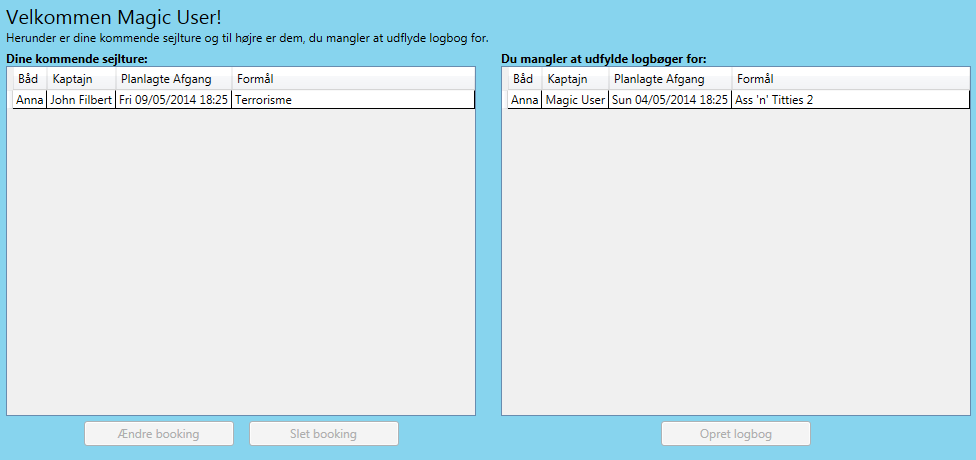
\includegraphics[scale=0.75]{UI/UserControl_FrontPage}
%    \end{center}
%    \vspace{-15pt}
%    \caption{Login interface}
%\end{wrapfigure}


\textbf{Datafremvisning:} 
En brugers kommende sejlture, og sejlture hvor brugeren mangler at udgylde logbøger for.

\textbf{Funktioner:} 
Kan åbne opret logbogsvinduet, enten ved dobbeltklik på sejltur, eller ved valgt af markering og tryk på opret logbog knappen. 

\textbf{Logik:} 
Hvis ingen sejltur er valgt i DataGridet med logbøger, så skal opret logbog knappen ikke være tilgængelig.

\fixme{Mangler billede, tænker at vi tager screenshots fra en platfor (win8/win7)}


\section{Vinduer}
\subsection{Opret sejltur}

\textbf{Datafremvisning:} 
Viser det data som bliver valgt, når brugeren vælger det. 
Der er også flere conscructorer, således der kan forudintastes data ved dets oprettelse.

\textbf{Funktioner:} 
Kan åbne vælg besætningsvinduet. 
Kan gemme data til databasen, hvis turen er gyldig.

\textbf{Logik:} 
Der verificeres om turen er gyldig, der er flere krav:
\begin{itemize}
    \item Er der valgt en båd?
    \item Er starttidspunktet efter det nuværende?
    \item Er sluttidspunktet efter starttidspunktet?
    \item Er båden ledig i dette tidsrum?
    \item Er der valgt mindst et besætningsmedlem?
    \item Er der valgt en kaptajn?
    \item Er der angivet et formål?
\end{itemize}


\subsection{CreateCrewWindow}

\begin{wrapfigure}{r}{0.5\textwidth}
    \label{img:login_interface}
    \vspace{-20pt}
    \begin{center}
        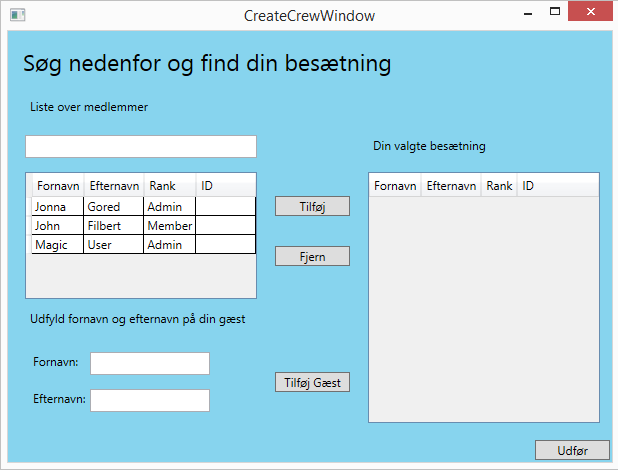
\includegraphics[width=0.48\textwidth]{Screenshots/CreateCrewWindow.png}
    \end{center}
    \vspace{-20pt}
    \caption{CreateCrewWindow}
    \vspace{-30pt}
\end{wrapfigure}

\textbf{Formål}: Dette vindue åbnes op to steder i programmet: \textbf{CreateLogbookWindow} og i \textbf{CreateBoatBookingWindow}. Det bruges når der skal laves en besætning til en RegularSailtrip.  

\textbf{BrugerGrænseflade}: Der er to datagrids som indeholder to lister. Listen til venstre består af SailClubMembers som bliver hentet ind fra databasen. Listen til højre indeholder det Crew som man er i gang med at udforme til enten RegularSailTrip, eller Logbook. Der er også tilføjet tekstfelter, så man kan skrive navnet på en gæst man tog med på sejlturen. Der er knapper som tilføjer de forskellige personer til Crewlisten. Øverst findes også et tekstfelt til at søge listen over medlemmer igennem. Når man har lavet sin liste, kan man trykke udfør, for at komme tilbage til vinduet der kaldte CreateCrewWindow.

\textbf{Code-Behind}: 
På \myref{AddGuestButton} kan man se koden der sker når man trykker på knappen med teksten Tilføj Gæst.
Der er blevet brugt et \textbf{regular expression} til at tjekke om den string brugeren angiver i de to tekstbokse for gæstens navne er lovlige. 
Det er blevet valgt man må bruge hele det danske alfabet samt mellemrum, så navne såsom: Lars Peter Vesterager, er mulige.
Hvis begge tekstbokse er lovlige, kommer man ind i det inderste if-statement, hvor der laves en ny person med det pågældende FirstName og LastName. 
Derefter tilføjes personen til Listen der vises i Datagridded til højre, og til sidst kaldes RefreshDatagrid, som man kan se på \myref{RefreshDatagrid}.

\begin{lstlisting}[frame=single, caption=Add Guest Buttton, label=AddGuestButton]
{
    if (Regex.IsMatch(FirstNameBox.Text, "^[A-ZÆØÅa-zæøå ]*$") && FirstNameBox.Text.Trim() != String.Empty)
    {
        if (Regex.IsMatch(LastNameBox.Text, "^[A-ZÆØÅa-zæøå ]*$") && LastNameBox.Text.Trim() != String.Empty)
        {
            var p = new Person();
            p.FirstName = FirstNameBox.Text;
            p.LastName = LastNameBox.Text;
            CrewList.Add(p);

            RefreshDatagrid(CurrentCrewDataGrid, CrewList);

            FirstNameBox.Clear();
            LastNameBox.Clear();
        }
    }
    else
    {
        MessageBox.Show("Ugyldigt navn. \nPrøv venligst igen");
    }
}      
\end{lstlisting}

Her modtages der et Datagrid, som skal have dets Itemssource Refreshet, og en ICollection, som er det data der skal sættes ind i Datagridded. 
Det gøres ved at assigne dets Itemssource til null, og derefter assigne det tilbage til den ICollection der blev sendt med. 

\begin{lstlisting}[frame=single, caption=Refresh Datagrid, label=RefreshDatagrid]
private void RefreshDatagrid(DataGrid Grid, ICollection<Person> list)
{
    Grid.ItemsSource = null;
    Grid.ItemsSource = list;
}
\end{lstlisting}

Knappen til at tilføje et medlem kan ses på \myref{AddMember}.
Inden det valgte medlem tilføjes til listen tjekkes der om medlemmet allerede findes i den anden liste. 
Dette gøres ved at anvende standard query operatorerne. 
Først et where med et lambda udtryk hvor der findes alle SailClubMembers i listen. 
Herefter castes disse om til SailClubMembers, for derefter at kunne tjekke om det valgte medlems SailClubMemberId er forskelligt fra de andre i listen. 
Hvis det hele er true, så bliver det valgte medlem tilføjet til listen, og RefreshDataGrid kaldes for at opdatere Datagridded.

\begin{lstlisting}[frame=single, caption=Add Member, label=AddMember]
private void AddButton_OnClick(object sender, RoutedEventArgs e)
{
    var currentPerson = (SailClubMember) MemberDataGrid.SelectedItem;

    if (
        CrewList.Where(x => x is SailClubMember)
            .Cast<SailClubMember>()
            .All(x => x.SailClubMemberId != currentPerson.SailClubMemberId))
        CrewList.Add(currentPerson);

    DataGridCollection.Filter = Filter; 
    RefreshDatagrid(CurrentCrewDataGrid, CrewList);
}
\end{lstlisting}

\subsection{CreateLogbookWindow}

\begin{wrapfigure}{r}{0.5\textwidth}
    \label{img:login_interface}
    \vspace{-20pt}
    \begin{center}
        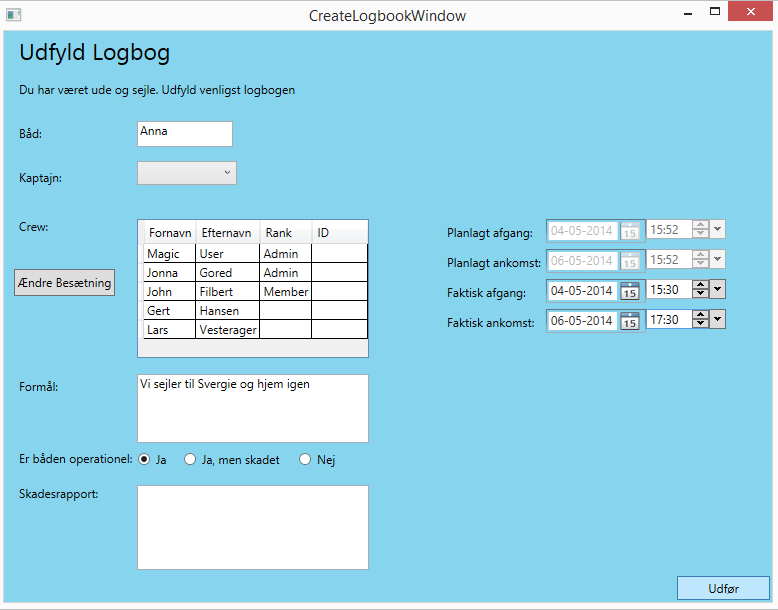
\includegraphics[width=0.48\textwidth]{Screenshots/CreateLogbook.png}
    \end{center}
    \vspace{-15pt}
    \caption{CreateLogBookWindow}
    \vspace{-30pt}
\end{wrapfigure}

\textbf{Formål}: Dette vindue bruges når et medlem som har booket en båd, skal udfylde sejlturens logbog. Vinduet tilgås fra usercontrollen FrontPage. Medlemmet skal udfylde de forskellige felter der findes i vinduet og trykke udfør, for at gemme logbogen i databasen.

\textbf{BrugerGrænseflade}: Der er mange elementer på dette skærmbillede. Øverst til venstre finder man en textbox, som udfyldes automatisk når man vil udfylde sin logbog. 
Textboxen indeholder navnet på den båd, logbogen skrives for, og dette loades igennem den RegularSailtrip, som logbogen skrives for.
Under den findes en combobox hvor man vælger Kaptajn eller bådføren for sejlturen.
Her kan vælges imellem alle de personer som er sat på besætningslisten. 
Der bliver altså ikke tjekket om personerne har duelighedsbevis, da gæsterne netop også kan være kaptajnen eller bådføren.
Under dette finder man en boks hvor man angiver turens formål. 
Der er desuden tre RadioButtons, som angiver hvilken tilstand båden er i. 
Hvis man aktivere enten knappen med teksten: "Ja men skadet" eller "nej", så påkræves det at man udfylder dette felt. 

Til højre finder man 4 DateTimePicker usercontrols, som beskrevet i \myref{subsec:DateTimePicker}. De to øverste er ikke enabled, da de også er loaded fra den RegularSailtrip man udfylder logbog for. De to andre skal dog udfyldes, og ændres fra de standardværdier som de har når man åbner vinduet. 

Under disse DateTimePickers, finder man endnu en textbox, som skal udfyldes med en vejrrapport.

Der findes et lignende vindue som hedder ViewSpecificLogbookWindow.
Dette vindue indeholder alle de samme felter, men har også et svar fra BoatChief som findes i en textbox.
Alle elementerne i det vindue er sat til Readonly eller IsEnabled="False", da man kun skal kunne se logbogen i det vindue, og altså ikke udfylde noget.


\textbf{Code-Behind}: Der er ikke meget kode at se på ved dette vindue, da meget af det er simpelt, men man kan se på den kode der findes bag knappen med teksten: "Udfør".
Koden for dette kan ses på \myref{SaveLogbookButton}.
Først tjekkes der om de forskellige felter i vinduet er udfyldt, og hvis alt er udfyldt kommer man ind i det sidste else if-statement der ses i koden. 
Her afsættes der om båden har taget skade under sejlturen, og derefter gemmes alle felterne i de lokale kopier af både RegularSailTrip og Logbook, hvor der til slut kaldes updateDatabase på de to lokale objekter.

\begin{lstlisting}[frame=single, caption= Gem Logbog, label=SaveLogbookButton]
private void FileLogbookButton_OnClick(object sender, RoutedEventArgs e)
{
	if (YesRadioButton.IsChecked == false && NoRadioButton.IsChecked == false)
	{
	    MessageBox.Show("Udfyld venligst om båden blev skadet under sejladsen");
	}
	...
	else if (YesRadioButton.IsChecked == true || NoRadioButton.IsChecked == true
	            || YesButBrokenRadioButton.IsChecked == true) 
	{
	        if (YesRadioButton.IsChecked == true)
	        {
	            currentLogbook.DamageInflicted = false;
	        }      
	        if (NoRadioButton.IsChecked == true || YesButBrokenRadioButton.IsChecked == true)
	        {
	            currentLogbook.DamageInflicted = true;
	        }
	    RegularSailTrip.PurposeAndArea = PurposeTextBox.Text;
	    currentLogbook.DamageDescription = DamageTextBox.Text;
	    currentLogbook.ActualCrew = CrewList;
	    currentLogbook.ActualArrivalTime = DateTimePickerActualArrival.Value;
	    currentLogbook.ActualDepartureTime = DateTimePickerActualDeparture.Value;
	    currentLogbook.FiledBy = _currentSailClubMember;
	    RegularSailTrip.WeatherConditions = WeatherConditionTextBox.Text;
	    RegularSailTrip.Crew = CrewList;
	    RegularSailTrip.Logbook = currentLogbook;
}
\end{lstlisting}

\fxnote{Opdater denne listning med Update Database kaldet.}

